\documentclass[bachelor, och, coursework, times]{SCWorks}
% параметр - тип обучения - одно из значений:
%    spec     - специальность
%    bachelor - бакалавриат (по умолчанию)
%    master   - магистратура
% параметр - форма обучения - одно из значений:
%    och   - очное (по умолчанию)
%    zaoch - заочное
% параметр - тип работы - одно из значений:
%    referat    - реферат
%    coursework - курсовая работа (по умолчанию)
%    diploma    - дипломная работа
%    pract      - отчет по практике
% параметр - включение шрифта
%    times    - включение шрифта Times New Roman (если установлен)
%               по умолчанию выключен
\usepackage{listings}
\usepackage[T2A]{fontenc}
\usepackage[cp1251]{inputenc}
\usepackage{graphicx}
\usepackage[sort,compress]{cite}
\usepackage{amsmath}
\usepackage{amssymb}
\usepackage{amsthm}
\usepackage{fancyvrb}
\usepackage{longtable}
\usepackage{floatflt}
\usepackage{array}
\usepackage[english,russian]{babel}


\usepackage[colorlinks=true]{hyperref}





\begin{document}

\lstset{ 
language=C++, 
basicstyle=\small, 
numbers=left, 
numberstyle=\tiny,
stepnumber=1, 
numbersep=5pt, 
%backgroundcolor=\color{white}, % ???? ???? ????????? - ?????????? \usepackage{color}
showspaces=false, % ?????????? ??? ??? ??????? ???????????? ?????????
showstringspaces=false, % ?????????? ??? ??? ??????? ? ???????
showtabs=false, % ?????????? ??? ??? ????????? ? ???????
frame=single, % ???????? ????? ?????? ????
tabsize=2, % ?????? ????????? ?? ????????? ????? 2 ????????
captionpos=t, % ??????? ????????? ?????? [t] ??? ????? [b] 
breaklines=true, % ????????????? ?????????? ?????? (??\???)
breakatwhitespace=false, % ?????????? ?????? ?????? ???? ???? ??????
escapeinside={\%*}{*)} % ???? ????? ???????? ??????????? ? ????
}

% Кафедра (в родительном падеже)
\chair{дискретной математики и информационных технологий}

% Тема работы
\worktitle{ RK серии ''Коннор'' для для помощи в расследовании дел, связанных с девиантными андроидами }

% Курс
\course{3}

% Группа
\group{321}

% Факультет (в родительном падеже) (по умолчанию "факультета КНиИТ")
%\department{механико"=математического факультета}

% Специальность/направление код - наименование
%\napravlenie{010300 "--- Фундаментальная информатика и информационные технологии}
%\napravlenie{010500 "--- Математическое обеспечение и администрирование информационных систем}
%\napravlenie{230100 "--- Информатика и вычислительная техника}
%\napravlenie{231000 "--- Программная инженерия}
\napravlenie{09.03.01 "--- Информатика и вычислительная техника}

% Для студентки. Для работы студента следующая команда не нужна.
%\studenttitle{Студентки}

% Фамилия, имя, отчество студента(ки) в родительном падеже
\studentName{Экгарт Викентия Александровича}

% Заведующий кафедрой
\chtitle{к.ф.-м.н. доцент} % степень, звание
\chname{Л.Б. Тяпаев}  % Инициалы и фамилия

%Научный руководитель (для реферата преподаватель проверяющий работу)
\satitle{ассистент} %должность, степень, звание
\saname{В. А. Поздняков}  % Инициалы и фамилия

% Руководитель практики от организации (только для практики,
% для остальных типов работ не используется)
\patitle{} %должность, степень, звание
\paname{}  % Инициалы и фамилия

% Семестр (только для практики, для остальных
% типов работ не используется)
\term{} % номер

% Наименование практики (только для практики, для остальных
% типов работ не используется)
\practtype{}

% Продолжительность практики (количество недель) (только для практики,
% для остальных типов работ не используется)
\duration{} % число недель

% Даты начала и окончания практики (только для практики, для остальных
% типов работ не используется)
\practStart{}  % в формате ДД.ММ.ГГГГ
\practFinish{} % в формате ДД.ММ.ГГГГ

% Год выполнения отчета
\year{2019}  % в формате ГГГГ

\MakeTitle


\tableofcontents

% Раздел "Введение"
\intro

Целью данной курсовой работы является разработка чат-бота, работающего с API социальной сети "Вконтакте" для помощи
старосте в оповещении студентов о различных мероприятиях и прочих объявлениях, 
а также для мгновенного получения акутальной информации о порядке текущей недели в расписании,
без необходимости ручного высчитывания или обращения к сторонним ресурсам.
Данная социальная сеть была выбрана, поскольку количество пользователей (в том числе и студентов ВУЗа) в ней максимально,
в отличае от других социальных сетей. Также, данная социальная сеть полностью поддерживает законодательство РФ.
%принудительный перенос, ибо латех почему-то не перенс
В работе будет рассмотрен полный путь от знакомста с API социальной сети и, до конечного запуска бота на сервере.

Для достижения поставленной цели необходимо решить следующие задачи: 
\begin {enumerate}
	\item Дать определение понятию <<API>>.
	\item Ознакомиться с официальной документацией API от выбранной социальной сети.
	\item Выбрать технологии для решения поставленной задачи.
	\item Разработать чат-бота.
\end {enumerate}
%TODO - убрать личные местоимения
\section{Понятие <<API>>}
API --- application programming interface, по русски - программный интерфейс приложения,
Т.е. это описание способов (набор определенных "открытых" методов с парамаетрами, констант для изменения)
которыми одно компьютерное программное обеспечение может взаимодействовать с другим компьютерным ПО. При этом, как правило, 
при хорошем проектировании API, не имеет значения на каком языке будет написана программа, которая будет обращаться к этому API. Так, например,
программа написанная на C++ может работать с API программы, написанной на Java.

Поскольку API --- это всегда некие договоренности между двумя командами разработки (backend и frontend),
то появилась необходимость введения некоего стандарта, который бы описывал взаимодействие
между клиентом и сервером. Введение такого стандарата позволило бы писать четко структурированный
код и упростило бы понимание того, какие методы есть у одной команды для другой.

Обычно, API отвечает на запрос к нему в неком формате. В последнее время это два популярных формата
XML и JSON. Ниже можно увидеть два одинаковых по смыслу и количеству информации ответы.

JSON
\begin{lstlisting}
  {
    "age" : 12,
    "name" : "Danielle"
  }
\end{lstlisting}

XML
\begin{lstlisting}
<person>
  <age>12</age>
  <name>Danielle</name>
</person>
\end{lstlisting}

Так как XML еще и выполняет функцию языка разметки, до именно для взаимодействия КЛИЕНТ-СЕРВЕР предпочтительнее
использовать JSON

\section{Ознакомление с официальной документацией API Вконтакте}
Итак, документация данной социальной сети находится по слудующему адресу
\href{https://vk.com/dev/manuals}{https://vk.com/dev/manuals}.

Для решения поставленной задачи, заходим в раздел с чат ботами, 
и видим, что для взаимодействия бота и сервера социальной сети предусмотрено два способа общения "клиент-сервер":

\begin{itemize}
  \item Callback API.
  \item Long Poll API.
\end{itemize}

Callback API --- согласно официальной документации,
работает следующим образом - как только в сообществе происходит нужное событие - от сервера
Вконтакте приходит уведомление на наш сервер. При этом, событие может быть каким угодно: комментарий к фотографии, новая запись на стене,
вступление в сообщество, отправка сообщения, и многое другое. \cite{VKBots}.

Второй способ получения обновлений --- это подключение к Long Poll серверу.
В отличие от Callback API, Long Poll сервер будет присылать на наш сервер только те обновления,
которые связаны с сообщениями. Никаких других событий из сообщества в нём нет.
В целом, Long Polling --- это технология, которая позволяет получать данные о новых событиях
с помощью «длинных запросов». Иначе говоря, сервер получает запрос, но отправляет ответ
на него не сразу, а лишь тогда, когда произойдет какое-либо событие
(например, придёт новое сообщение), либо истечет заданное время ожидания. 
Используя этот подход, Вы можете мгновенно отображать в своем приложении важные события.
Чтобы использовать Bots Long Poll API, нужно 
открыть раздел «Управление сообществом» и на вкладке
«Работа с API»→«Long Poll API» выбрать «Включён».


Исходя из поставленной задачи, а также из-за некоторых преимуществ в скорости Long Poll API над обычным \cite{LongPoll}, принято решение использовать Long Poll API.

Также, необходимо создать сообщество в социальной сети Вконтакте, от имени которого будет писать чат бот.

\section{Выбор технологии для решения поставленной задачи}
Выбранный мною функционал чат-бота предполагает следующий сценарий использования :
Создатель беседы (беседа - чат между несколькими пользователями) или любой другой её участник добавлеят бота в беседу.
Далее администатор беседы открывает боту доступ ко всем сообщениям в ней и делает бота администратором 
(необходимо для работы функции "позови всех")

После этого доступны следующие команды боту :
\begin{itemize}
  \item какая неделя [сейчас, завтра, следующая]
  \item позови всех
  \item объявление
  \item инфо, помощь, что ты умеешь
\end{itemize}

Первая команда должна вернуть информацию о том,
какая сейчас (или иная, зависит от запроса пользователя) неделя.
Например, бот может ответить "сейчас числитель",
что означает что в данный момент актуальны пары из верхних ячеек расписания.

Вторая команда "позови всех" отправляет каждому пользователю уведомление,
даже если уведомления у этого пользователя отключены. Полезно, так как многие пользователи в виду
частых и неинфрмативных сообщени (флуд) отключают уведомления из беседы и могут пропустить что-то важное.

Третья команда "объявление" --- отправляет каждому пользователю уведомление с текстом, идущем после этой команды.
Работет даже если уведомления у этого пользователя отключены. Как в случае и с предидущим пунктом,
защищает пользователей от несвоевременного информирования при отключенных уведомлениях.

Последняя команда выводит информацию о доступных командах на данный момент.

Основываясь на вышеизложенных требованиях, а также на том, что бот будет обращаться
с сервером социальной сети через LongPoll API, можно выделить следующие технологии и языки
программирования, которые помогут решить поставленную задачу:

\begin{itemize}
  \item Java SDK
  \item PHP SDK
  \item Node.js SDK
\end{itemize}

Поскольку в боте не будет коммерческой составляющей, а также не потребуется работать с ценами и 
делать различного рода транзакции, то Java не подойдет из-за её громоздкости. Ведь для простой команды,
в стиле "привет, бот", в Java потребуется написать кучу классов и придется имплиментировать интерфейсы, 
даже если мне не будут нужны все остальные фукнции.

Что касается PHP и NodeJS \cite{PHP} --- по своей концепции они оба интерпретируемые.
Одинаково просты в освоении, но по скорости работы выигрывает PHP. Так как не предполагается, что
ботом будут пользоваться огромное количество народа, то данное примущество не слишком влияет на выбор.
А вот неблокирующий IO у NodeJS --- очень хорошее приемущество. \cite{IO} Ведь это означает, что процесс может
продолжить выполение не дожидаясь окончания передачи данных. С помощью этого, можно будет делать запросы
к сторонним API внутри бота (например, о погоде), получать данные и отдавать их дальше по цепочке для
отправки конечному пользователю социальной сети.


В итоге, для достижения полного механизма работы мной были выбраны следующие технологии:
\begin{enumerate}
 
  \item enviroment.
  \begin {itemize}
	\item Node JS. (серверный интрператор JS)
	\item PM2. (перезапуск процесса в случае ошибки, а также более продвинутое логирование)
  \end {itemize}
  \item bot.
  \begin {itemize} 
  	\item NPM (пакетный менеджер для работы с зависимостями).
  	\item vk-node-sdk (библиотека для взаимодействием с LongPoll API).
  	\item util (библиотека для логирования ошибок)
  	\item JavaScript (язык программирования).
  \end {itemize}
  \item Сервер.
  \begin {itemize}
	\item Ubuntu 17.10 64bit (512 МБ RAM 20 ГБ SSD 1 CPU).
  \end {itemize} 
\end{enumerate}

Посльку не требуется хранить какие-либо данные, полученные от пользователя, база данных не учавствует в проекте.

В качестве IDE была использована VS Code от \copyright Microsoft.
Данная IDE имеет встроенную поддержку JavaScript, системы контроля версий, а также распространяется бесплатно.
\section {Разработка чат бота}
Разработка велась в три этапа --- программирование и создание серверной части - самого бота,
загрузка проекта на сервер и ручное тестирование функционала.
\subsection {чат-бот}
С помощью CLI (command line interface)
была создана директория для разрабтки и далее была введена команда `npm init` ,
которая создает конфигурационный файл трбуемого приложения. Полученный файл оказался таким

\begin{lstlisting}
    
  {
    "name": "bot_vk",
    "version": "1.0.0",
    "description": "konnor testing",
    "main": "konnor.js",
    "dependencies": {
      "node-vk-bot": "1.2.1",
      "util": "^0.11.0",
      "vk-node-sdk": "^0.1.8",
    },
    "scripts": {
      "test": "echo \"Error: no test specified\" && exit 1"
    },
    "author": "",
    "license": "ISC"
  }
\end{lstlisting}

Далее, был создан главный js файл --- "konnor.js",
в котором необходимо с помощью библиотеки "vk-node-sdk" подключиться к серверверу Вконтакте для приёма уведомлений.

Для этого, создал файл с константами, где будут указаны токены для работы с ботом, а также
ID сообщества, от чьего имени будет отвечать бот. Разнесение архитектуры приложения на несколько файлов
упростит его поддежку в дальнейшем и поможет делать важные изменения без затрагивания большого количства
кода.

Вот как выглядит данный файл сейчас:

\begin{lstlisting}
  const vkGroupFullRight = 'group on vk token fith full rights and long-poll';
  const groupId = 000;

  module.exports = {
      vkGroupFullRight: vkGroupFullRight,
      groupId: groupId,
  }
\end{lstlisting}

В главном файле, импортируем этот файл и инициализируем бота.

\begin{lstlisting}

const DEBUG_MODE = require('./konnor_config');
const util = require('util');
const { Bot } = require('node-vk-bot');

//don't forget to add tokens in file and rename him
const TOKENS = require('./secret_tokens');

const regName = /коннор|connor|конор|андроид/i;


const debugConsole = (variable, depth) => {
    DEBUG_MODE && console.log('debug: ' + util.inspect(variable, false, depth = 8));
}

const bot = new Bot({
    token: TOKENS.vkGroupFullRight,
    group_id: TOKENS.groupId,
}).start()

console.log('bot started');


bot.on('poll-error', error => {
    console.error('error occurred on a working with the Long Poll server ' +
        `(${util.inspect(error)})`)
})

\end{lstlisting}

Для запуска бота введем команду "node ./konnor.js". Бот запущен!

Прежде чем писать реакцию на команды, в соотвествии с принципами "Банды четырех" \cite{Gang} --- 
выносим каждую команду в отдельный модуль и делаем "горячее подключение" модулей. То есть не требуется 
переписывать общую логику бота, при добавлении новой команды в будущем.

Каждая команда - это объект, вида:
\begin{lstlisting}
  const имя_команды = {
    callName: 'триггер срабатывания, может быть регулярным выражением',
    action: (bot, message, TOKENS) => {
      дейсвие - что она делает
    }
}
\end{lstlisting}

Также, подключение команд реализуем в отдельном файле, дабы не трогать основной.

Сама же логика бота - на какую команду он среагирует будет осуществляться
следующим образом --- бот получает список всех доступных команд и входящее сообщение.
Далее простым циклом проходясь по списку команд, он сверяет "триггер" (регулярное выражение)
каждой команды с входным сообщением. И если регулярное выражение проходит (результат true),
то бот исполняет нужную команду и передаёт свой ответ на отправку.

Данный паттерн называется "Стратегия" и очень сильно экономит ресуры и облегчает
добваление новых команд. \cite{Stoyan}

Теперь реализуем действие на событие "новое сообщение" - для этого напишем в функции "on.message"
указанный сверху цикл. И добавим fallback - сообщение, которое отправится, если никакая команда не сработает.

\begin{lstlisting}
  bot.get(/./, message => {
    if (message.peer_id > 1000000000) { //message from conversation
        if (!regName.test(message.text)) { //if no name calling - no answeer
            return;
        }
    }
    bot.api('messages.setActivity', { type: 'typing', peer_id: message.peer_id, group_id: TOKENS.groupId })
        .then(res => console.log(util.inspect(res)));

    message.text = message.text.replace(regName, ''); //delete him name

    for (let skillName in skillList) {
        const regExp = RegExp(skillName, 'i');
        if (regExp.test(message.text)) {
            console.log('matched: ' + skillName);
            skillList[skillName](bot, message, TOKENS);
            return;
        }
    }

  })


\end{lstlisting}

На 7-8 строчках утсанавливаем статус "набирает сообщение" --- что придаст
боту больше человечности и будет понятно, что он получил сообщение и готовиться на него ответить.

Со 2 по 6 строки, проверяем, обращались ли к нему по имени, потому что данная функция будет
вызываться при любом сообщении из беседы, даже тогда, когда от бота ничего не требуется.


Ниже приведены три необходимых "навыка" бота для достижения цели этой работы.

Для призыва всех людей в беседу:
\begin{lstlisting}
  const mentionAll = {
    callName: 'позови всех',
    action: (bot, message, TOKENS) => {
        bot.api('messages.getConversationMembers', { peer_id: message.peer_id, group_id: TOKENS.groupId })
            .then(res => {
                //const usersNamesOrIds = res.profiles.map(profile => profile.screen_name != '' ? profile.screen_name : profile.id );
                //console.log(util.inspect(usersNamesOrIds));
                const mentionIds = res.profiles.map(profile => `@id${profile.id}`);
                bot.send('я призываю всех ' + `${mentionIds.toString()}`, message.peer_id).catch(
                    function (e) {
                        console.log(e);
                    }
                );
            })
            .catch(
                function (e) {
                    console.log(e);
                }
            );
    }
}

module.exports = mentionAll;
\end{lstlisting}

Для расылки всем объвления:
\begin{lstlisting}
  const sendMessageAll = {
    callName: 'об[ъь]явление',
    action: (bot, message, TOKENS) => {
        const alertMessage = message.text
                .split(/об[ъь]явление/i, 2)[1]
                .trim();
            bot.api('messages.getConversationMembers', { peer_id: message.peer_id, group_id: TOKENS.groupId })
                .then(res => {
                    const mentionIds = res.profiles.map(profile => `@id${profile.id}`);
                    bot.send(`сообщение для всех: ${alertMessage} ${mentionIds.toString()}`, message.peer_id).catch(
                        function (e) {
                            console.log(e);
                        }
                    );
                })
                .catch(
                    function (e) {
                        console.log(e);
                    }
                );
    }
}

module.exports = sendMessageAll;
\end{lstlisting}

Для определения числитель или знаменатель:
\begin{lstlisting}
      
const chislOrZnam = require('./logic');

const weekPair = {
    callName: 'какая неделя|неделя какая',
    action: (bot, message) => {
        let d = new Date();
        d.setHours(d.getHours() + 1); //for GMT+4
        
        let parity = 'сейчас ' + chislOrZnam(d);
        
        if (/завтра/i.test(message.text)) {
            d.setDate(d.getDate() + 1);
            parity = 'завтра ' + chislOrZnam(d);
        }
        if (/следующая/i.test(message.text)) {
            d.setDate(d.getDate() + 7);
            parity = 'следующая неделя ' + chislOrZnam(d);
        }
        bot.send(parity, message.peer_id).catch(
            function (e) {
                console.log(e);
            }
        );
    }
}

module.exports = weekPair;
\end{lstlisting}

Логика опредения числителя и знаменателя - смотрите в приложении.


\subsection {Развертка приложения на сервере}

\subsubsection {Покупка сервера}
Прежде всего необходимо купить сервер.

Для этого, идем на сайт \href{https://vscale.io/panel/scalets/}{https://vscale.io/panel/scalets/} и 
жмём кнопку 'создать сервер'. 
\begin{figure}[h]
  \center{
\includegraphics[width=1\linewidth]{pair.jpg}}
  \caption{Запрос с целью узнать, какая неделя в расписании будет актуальна завтра.}
  \label{ris:pair}
  \end{figure}


\subsubsection {Использование сервера}
Далее необходимо подключиться к серверу по SSH и
склонировать туда репозиторий проекта, установить все пакеты и запустить.


Установим библиотеку PM2  глобально с помощью менеджера пакетов NPM:

\begin{lstlisting}
  npm i pm2 -g
\end{lstlisting}

Далее, запустим бота командой: 

\begin{lstlisting}
  pm2 start konnor.js
\end{lstlisting}

Теперь, терминал можно зыкрывать - бот запущен и работет.


Для того, чтобы смотреть логи, нужно использовать команду:

\begin{lstlisting}
  pm2 logs konnor
\end{lstlisting}


\subsection {Ручное тестирование бота}

Поскольку предполагается, что чат-ботом будут пользоваться люди, можно ожидать, что
кроме доступных команд, они будут пытаться отправить роботу картинки, символы не из юникода и прочее.
При этом, бот не должен падать или зависать, а должен лишь строго реагировать на команды.\cite{Test}

После тестирования, ошибок не было выявлено.

Ниже на Рисунке~\ref{ris:pair} и Рисунке~\ref{ris:all} приведены скриншоты успешной работы бота.

\begin{figure}[h]
\center{
\includegraphics[width=1\linewidth]{pair.jpg}}
\caption{Запрос с целью узнать, какая неделя в расписании будет актуальна завтра.}
\label{ris:pair}
\end{figure}

\begin{figure}[h]
\center{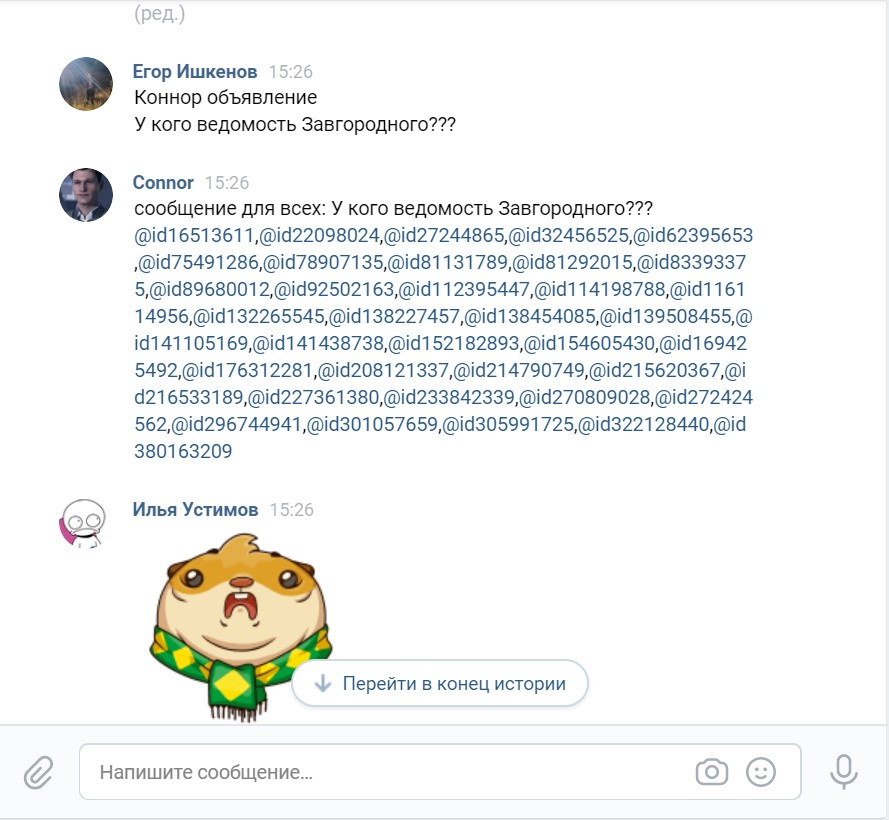
\includegraphics[width=1\linewidth]{all.jpg}}
\caption{Староста использует возможности бота, чтобы очень быстро обратиться ко всем с важным вопрсом.}
\label{ris:all}
\end{figure}

%на рисунках 1 и 2 скриншоты приложения

\section {\appendixname}
\appendix {Функция для определения порядка текущей недели - числитель или знаменатель. Используется в модуле
'какая неделя?'}

\begin{lstlisting}
  const chislOrZnamen = (date) => {
    let now = new Date();
    if (date) {
        now = date;
    }
    //изначально считаем что сейчас числитель
    //true - числитель
    //false - знаменатель
    
    const dayFirstOfSeptember = (new Date(now.getFullYear(), 8, 1)).getDay();
    const dateFirstMondayInSeptember = (dayFirstOfSeptember == 2) ? 7 : (9 - dayFirstOfSeptember) % 7;
    
    const dayFirstOfJanuary = (new Date(now.getFullYear(), 0, 1)).getDay();
    const dateFirstMondayInJanuary = (dayFirstOfJanuary == 2) ? 7 : (9 - dayFirstOfJanuary) % 7;
    
    const currentDate = now.getDate();
    const currentMonth = now.getMonth();
    
    const countFullWeeksBeforeNY = Math.floor((now.getTime() - new Date(now.getFullYear(), 8, dateFirstMondayInSeptember).getTime()) / 86400000 / 7);
    const countFullWeeksAfterNY = Math.floor((now.getTime() - new Date(now.getFullYear(), 0, dateFirstMondayInJanuary).getTime()) / 86400000 / 7);
    
    if (currentMonth > 8 && countFullWeeksBeforeNY % 2 != 0) {
        return 'числитель'
    }
    else if (currentMonth == 8) {
        if (currentDate >= dateFirstMondayInSeptember && countFullWeeksBeforeNY % 2 != 0) {
            return 'числитель'
        }
        else if (currentDate < dateFirstMondayInSeptember) {
            return 'числитель'
        }
    }
    else if (currentMonth < 8) {
        if (currentMonth <= 4 && currentMonth >= 0) {
            if ((currentMonth == 0) && (currentDate < dateFirstMondayInJanuary)) {
                if (dayFirstOfSeptember == 0 || dayFirstOfSeptember > 4) {
                    return 'числитель'
                }
            }
            else if (countFullWeeksAfterNY % 2 == 0) {
                return 'знаменатель'
            }
        }
        else if (currentMonth > 4) {
            console.log('сейчас лето, ты чего');
        }
    }
    return 'числитель'
}

module.exports = chislOrZnamen;
\end{lstlisting}

\conclusion 
При выполнении данной курсовой работы,
было проведено ознакомление с понятнием API, а также
была изучена официальная документация социальной сети для
написания ботов и были выполнены поставленные задачи по облегчению
управления беседой для старосты.

Исходный код приложения доступен в репозитории GitHub: 

https://github.com/vikegart/konnor

В дальнейшем планируется внедрить распознавание речи, в целях облегчения пользования чатом для людей,
которым прослушивание голосовых сообщений затруднительно.
\begin{thebibliography}{99}
  \bibitem{LongPoll} Bots Long Poll API [Электронный ресурс]: URL: https://vk.com/dev/bots\_longpoll (Дата обращения: 18.02.2019) Загл. с экрана. Яз. англ;
  \bibitem{VKBots} API для чат-ботов [Электронный ресурс]: URL: https://vk.com/dev/bots\_docs (Дата обращения: 18.02.2019) Загл. с экрана. Яз. англ;
  \bibitem{PHP} PHP vs NodeJS Comparison and Benchmark [Электронный ресурс]: URL: https://thinkmobiles.com/blog/php-vs-nodejs/ (Дата обращения: 19.02.2019) Загл. с экрана. Яз. англ;
  \bibitem{IO} Synchronous and Asynchronous I/O [Электронный ресурс]: URL: https://docs.microsoft.com/ru-ru/windows/desktop/FileIO/synchronous-and-asynchronous-i-o (Дата обращения: 19.02.2019) Загл. с экрана. Яз. англ;
  \bibitem{Gang} Приемы объектно-ориентированного проектирования. Паттерны проектирования.  Влиссидес Джон , Джонсон Р. , Хелм Ричард , Гамма Эрих Яз. англ стр [50-120];
  \bibitem{Stoyan} JavaScript. Шаблоны . Стоян Стефанов Яз. рус. стр [70-90];
  \bibitem{Test} Тестирование dot com . Савин Роман Яз. рус. стр 158;
\end{thebibliography}


\end{document}
